%% This is an example first chapter.  You should put chapter/appendix that you
%% write into a separate file, and add a line \include{yourfilename} to
%% main.tex, where `yourfilename.tex' is the name of the chapter/appendix file.
%% You can process specific files by typing their names in at the 
%% \files=
%% prompt when you run the file main.tex through LaTeX.

\chapter{Conceptos Básicos}

\clearpage
\section{Publicidad en internet}

La publicidad en internet se hace a base del contenido de la pagina web. Para el desarrollo de este tipo de publicidad que tiene como fin dar a conocer por medio de este formato un producto a los usuarios en línea se incluyen elementos como texto, enlaces, imágenes, animaciones, etc. Existen compañías como Google que han creado sistemas para la publicad en internet en este caso AdSense y AdWords \cite{kowaliw2012promoting}, este sistema coloca la publicidad que se desea mostrar en los sitios relacionados con el tema del producto que se desea promocionar y se especifica el precio a pagar por cada clic del usuario a la publicidad. El sitio web que tiene anuncios al rededor de su contenido obtendrá ganancias según la cantidad de clics y el precio que se allá fijado para cada uno de los anuncios, El anunciante obtendrá mayor trafico en su sitio donde dispone del producto que anuncia, y así se logra la publicidad.

\clearpage
\section{Article spinning}

Article spinning es un método para crear múltiples versiones de un articulo sin crear versiones consideradas plagio ya que cada versión es única. El contenido duplicado no es aceptado por los motores de búsqueda como Google, Yahoo y Bing, así que este método se utiliza para generar muchos artículos basándose en uno solo, las palabras del articulo son sustituidas  por sinónimos automáticamente y se crea otra versión del articulo, esto ayuda a evitar las sanciones en las páginas de resultados de los motores de búsqueda ( SERP ) para el uso de contenido duplicado.\cite{takagi2001interactive}.

Existe gran similitud en el funcionamiento del "Article Spinning" con el de una máquina tragamonedas. Como se puede observar en la figura \ref{as}, podemos tener varias letras que pueden ser sustituidas en la primera ventana de la máquina tragamonedas. En este caso, esas letras son W, F y L, y representan bloques de texto. Al jalar la palanca, sólo una de de esas letras ganará la posición. La decisión de quién ganará la posición es aleatoria. Una vez que se jale la palanca (que sería el equivalente a accionar un botón para generar una combinación de palabras, y así crear un articulo nuevo) se genera una combinación de letras, que en este ejemplo fue la letra W, I y la letra N, las cuales juntas se puede leer como WIN (en español significa ganar).


\begin{figure}[htp]
  \centerline{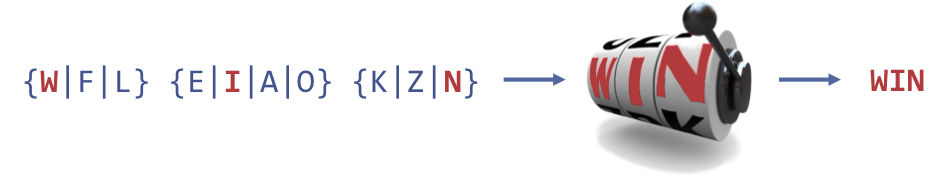
\includegraphics[width=4.5in]{as.png}} 
  \caption{funcionamiento del Article Spinning} 
\label{as}
\end{figure}

\clearpage
\section{Algoritmos Evolutivos}

Los algoritmos evolutivos son una rama de la inteligencia artificial, se utilizan principalmente en problemas con espacios de búsqueda muy extensos y no lineales. Estos algoritmos buscan soluciones basadas en la teoría de la evolución darwiniana. 
Con este método se mantiene un conjunto de individuos que representan posibles soluciones, estas soluciones se mezclan, y compiten entre si, de esa forma las soluciones mas aptas son capaces de sobrevivir a lo largo del tiempo y contribuir a las siguientes generaciones aportando sus genes, de esa forma estas generaciones venideras irán evolucionando hacia mejores soluciones cada vez. Existen distintos algoritmos evolutivos pero el que tiene mas importancia para esta investigación es el algoritmo genético da-do que es el que utilizamos para resolver nuestro problema.\cite{malcolm2008approach}

\clearpage
\subsection{Algoritmos Genéticos}

Los algoritmos genéticos (AG) (en la figura \ref{diagrama} podemos observar el diagrama de un AG) se inspiran en la evolución biológica, hacen evolucionar una población de individuos sometiéndola a mutaciones y recombinaciones genéticas, también a una selección de acuerdo a algún criterio, en función de este criterio se deciden cuales son los individuos más aptos, los cuales sobreviven y los menos aptos que son descartados. Es un método de búsqueda dirigida basada en probabilidad.\cite{back1996evolutionary}

Los algoritmos geneticos, consisten en una funcion matematica o una rutina que Simula el proceso evolutivo de las especies, teniendo como objetivo encontrar soluciones a problemas especificos de maximizacion o minimizacion. Asi, el algoritmo genetico recibe como entrada una generacion de posibles soluciones para el problema en cuestion, y arroja como salida los especimenes mas aptos (es decir, las mejores soluciones), para que se apareen y generen descendientes, los que deberian tener mejores caracteristicas que las generaciones anteriores.

Estos algoritmos mantienen elitismo ya que guarda siempre al mejor elemento de la población sin modificarlo. Al aumentar el numero de iteraciones, la probabilidad de encontrar el resultado optimo tiende a uno.

Los algoritmos geneticos trabajan con codigos que representan las posibles soluciones al problema. Por ello, es necesario establecer una codificacion para todo el rango de posibles soluciones antes de comenzar a trabajar con el algoritmo.La codificacion mas utilizada es la representacion de las soluciones por medio de cadenas binarias.\cite{parisi2004modelos}

\begin{figure}[htp]
  \centerline{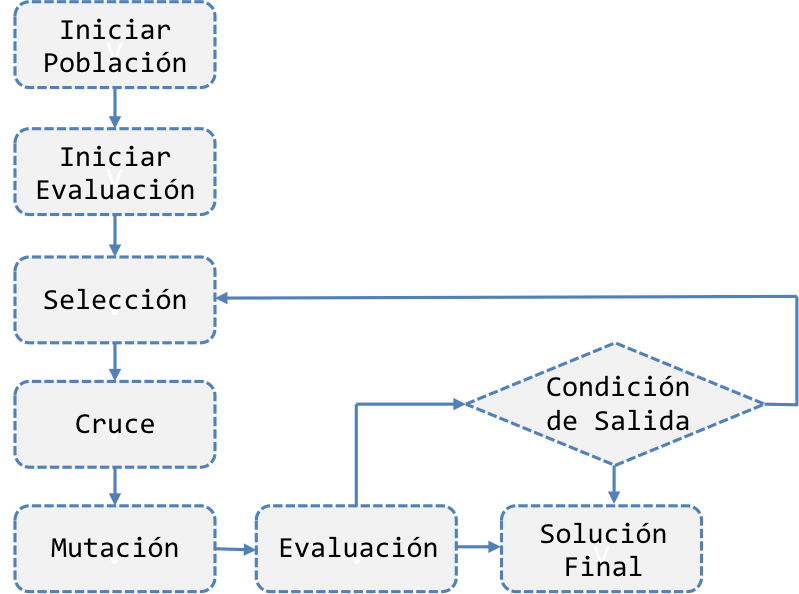
\includegraphics[width=4in]{diagrama.png}} 
  \caption{Diagrama de un Algoritmo Genético} 
\label{diagrama}
\end{figure}

\clearpage
\subsection{Computación Evolutiva Interactiva}

La computación evolutiva interactiva es una variación de la computación evolutiva en la cual la aptitud del individuo se determina mediante una evaluación subjetiva realizada por un usuario humano. En la computación tradicional, un humano requiere de un proceso computacional para resolver un problema, proporcionando la descripción del problema obtiene un resultado que después interpreta, pero en la computación evolutiva interactiva se invierten los papeles, existe un algoritmo que pide a un humano o a un grupo de humanos que resuelvan un problema, después recopila las soluciones para poder interpretarlas.\cite{dao2012novel}

Estos algoritmos se utilizan principalmente en problemas de optimización en el que el espacio de búsqueda es muy grande y complejo. Estos algoritmos de búsqueda de soluciones basadas en la teoría de la evolución darwiniana.
 
Este tipo de métodos de optimización generan un conjunto de individuos que representan posibles soluciones. Estas soluciones normalmente se generan al azar al comienzo del proceso de evolución. Después de cada generación, las mejores soluciones comparten parte de su información para crear otras posibles mejores soluciones. Todos los individuos compiten para ser la solución mas apta; las mejores soluciones se conservan, mientras que las peores son destruidos, de acuerdo con una función de aptitud que evalúa su rendimiento \cite{back1996evolutionary}. 

La computación evolutiva interactiva (CEI) utiliza una función de aptitud que se determina mediante la evaluación subjetiva de un ser humano, por ejemplo, una persona que está considerando un anuncio de texto para ser mejor que otro.

\clearpage
\section{EvoSpace}

Evospace es un espacio o hábitat en la nube donde se pueden almacenar y desarrollar algoritmos evolutivos. Evospace es muy versátil ya que la población es  independiente al modelo evolutivo que se pretenda utilizar. Los procesos clientes llamados EvoWorkes, interaccionan dinámica y asíncronamente, ellos también puede desplegarse en clientes remotos como en la plataforma que alberga al servidor.\cite{garcia2013evospace}